\documentclass[tikz,border=10pt]{standalone}
% No extra TikZ libraries needed for this figure.
\begin{document}
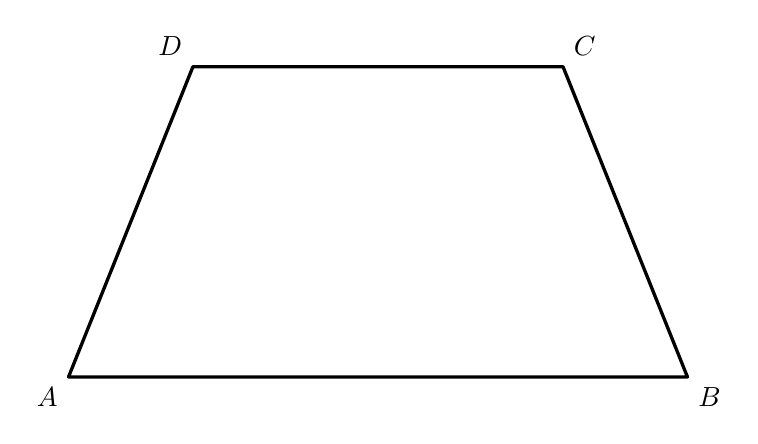
\begin{tikzpicture}[line width=1.2pt, line join=round]
  % Vertices: pixel coords converted with s = 0.02 cm/px,
  % centre (263.9, 144.5) px mapped to the origin, y flipped.
  \coordinate (A) at (-3.93,-1.97);  % px (67.4, 243.0)
  \coordinate (B) at ( 3.93,-1.97);  % px (460.4, 243.0)
  \coordinate (C) at ( 2.35, 1.97);  % px (381.6, 46.0)
  \coordinate (D) at (-2.35, 1.97);  % px (146.4, 46.0)

  % Trapezoid edges AB, BC, CD, DA (solid)
  \draw (A) -- (B) -- (C) -- (D) -- cycle;

  % Vertex labels placed outside each corner
  \node[below left]  at (A) {$A$};
  \node[below right] at (B) {$B$};
  \node[above right] at (C) {$C$};
  \node[above left]  at (D) {$D$};
\end{tikzpicture}
\end{document}